\RequirePackage{iftex}
\ifXeTeX
\else
    \GenericError{}{编译错误：本模板必须使用 XeLaTeX 编译！}
    {请将编译器切换为 XeLaTeX 重新编译。}{}
    \stop
\fi

\documentclass[openany]{book}

% ==================== 基础宏包 ====================
\usepackage[UTF8]{ctex}
\usepackage{graphicx,xcolor,tocloft}
\usepackage{fancyhdr,geometry,titlesec}
\usepackage{amsmath,amssymb}
\usepackage{tikz}
\usepackage{amsthm}
\usepackage{enumitem}
\usepackage{silence}
\usepackage{array}

% ==================== 页面边距与颜色 ====================
\geometry{
    left=2cm,
    right=2cm,
    top=2cm,
    bottom=2cm
}

\definecolor{myblue}{RGB}{0,83,159}

% ==================== 字体警告处理 ====================
\WarningFilter{latexfont}
{Font shape `TU/FandolSong-Regular(0)/b/it' undefined}

% ==================== 定理环境设置 ====================
\newtheoremstyle{mydefinition}
  {\topsep}
  {\topsep}
  {}
  {0pt}
  {\heiti\bfseries}
  {.}
  {.5em}
  {}

\newtheoremstyle{myplain}
  {\topsep}
  {\topsep}
  {}
  {0pt}
  {\heiti\bfseries}
  {.}
  {.5em}
  {}

\theoremstyle{mydefinition}
\newtheorem{definition}{定义}
\newtheorem{example}{例}

\theoremstyle{myplain}
\newtheorem{theorem}{定理}
\newtheorem{lemma}[theorem]{引理}
\newtheorem{corollary}[theorem]{推论}
\newtheorem{proposition}[theorem]{命题}

% ==================== 目录设置 ====================
\renewcommand{\cfttoctitlefont}
{\hfill\color{myblue}\heiti\Large}

\renewcommand{\cftaftertoctitle}{\hfill}

\renewcommand{\cftpartpagefont}{}
\renewcommand{\cftpartafterpnum}{\hspace{0pt}}
\renewcommand{\cftchapfont}{\normalfont}
\renewcommand{\cftsecfont}{\normalfont}
\renewcommand{\cftsubsecfont}{\normalfont}

\setlength{\cftbeforetoctitleskip}{-0.5em}
\setlength{\cftaftertoctitleskip}{0.5em}
\setlength{\cftbeforechapskip}{3pt}
\setlength{\cftbeforesecskip}{0pt}
\setlength{\cftbeforesubsecskip}{0pt}

% ==================== 页眉页脚 ====================
\setlength{\headheight}{15pt}

\pagestyle{fancy}
\fancyhf{}

\fancyhead[LE,RO]
{\color{myblue}\leftmark}

\fancyfoot[LE,RO]
{\color{myblue}\thepage}

\renewcommand{\headrule}
{{\color{myblue}\hrule height 0.4pt width\headwidth}}

\renewcommand{\footrule}
{{\color{myblue}\hrule height 0.4pt width\headwidth}}

\fancypagestyle{plain}{%
    \fancyhf{}%
    \fancyhead[LE,RO]
    {\color{myblue}\leftmark}%
    \fancyfoot[LE,RO]
    {\color{myblue}\thepage}%
    \renewcommand{\headrule}
    {{\color{myblue}\hrule height 0.4pt width\headwidth}}%
    \renewcommand{\footrule}
    {{\color{myblue}\hrule height 0.4pt width\headwidth}}%
}

% ==================== 总标题格式 ====================
\titleformat{name=\chapter,numberless}
    {\color{myblue}\heiti\Large\centering}
    {}
    {0pt}
    {}

\titlespacing*{\chapter}
{0pt}{-4em}{1em}

% ==================== 一级标题格式 ====================
% 四种方法分别编号为 1、2、3、4
\renewcommand{\thesection}{\arabic{section}}

\titleformat{\section}
    {\color{myblue}\heiti\large}
    {\thesection}
    {0.5em}
    {}

\titlespacing*{\section}
{0pt}{0.8em}{0.5em}

% ==================== 二级标题格式 ====================
% 编号形式为 3.1、3.2、4.1 等
\renewcommand{\thesubsection}
{\thesection.\arabic{subsection}}

\titleformat{\subsection}
    {\color{myblue}\heiti\normalsize}
    {\thesubsection}
    {0.5em}
    {}

\titlespacing*{\subsection}
{0pt}{0.7em}{0.5em}

% ==================== 图题设置 ====================
\renewcommand{\figurename}{图}

% ==================== 表格格式 ====================
\renewcommand{\arraystretch}{1.4}

% ======================================================
%                       正文开始
% ======================================================
\begin{document}

% ==================== 封面 ====================
\begin{titlepage}
    \thispagestyle{empty}
    \centering

    \vspace*{2cm}

    {\color{myblue}\rule{\textwidth}{2pt}}\par

    \vspace{1.5cm}

    {\color{myblue}\Huge
    \textbf{电输运测量方法}}\par

    \vspace{0.5cm}

    {\color{myblue}\Large
    两端法、四端法、霍尔棒法与范德堡法}\par

    \vspace{1.5cm}

    {\color{myblue}\rule{\textwidth}{2pt}}\par

    \vspace{4cm}

    {\Large Ethan}\par

    \vspace{0.5cm}

    {\large 2026年10月}\par

    \vfill
\end{titlepage}

% ==================== 目录 ====================
\setcounter{page}{1}
\tableofcontents
\newpage

% ======================================================
%                     电输运测量方法
% ======================================================

\vspace*{-0.5cm}

\begin{center}
    {\color{black}\heiti\Huge 电输运测量方法}
\end{center}

\vspace{0.3em}

\addcontentsline{toc}{chapter}{电输运测量方法}
\markboth{电输运测量方法}{}

\setcounter{section}{0}

% 从 0 开始，使四种方法自动编号为 1、2、3、4
\setcounter{section}{0}

\section{两端法}
% ======================================================
% 1 两端法
% ======================================================

两端法（two-terminal method）是最基本的电阻测量方式。
样品两端分别连接两个电极，同一对电极同时承担电流加载和电压测量。
测量时在两个电极之间通入电流 \(I\)，并记录两端电压 \(V\)，
由电压与电流的比值得到样品的两端电阻：

\[
R_{\mathrm{2P}}=\frac{V}{I}.
\]

两端法的主要特点是测量回路中包含电极--样品接触界面，
因此实验结果会受到接触电阻的影响。
对于接触电阻较大或样品本身电阻较小的情况，
这种影响尤其明显。

两端法与四端法的核心区别在于：
两端法中电流端与电压端没有分离，
因此测得的电压中可能包含电极--样品界面产生的额外电压降。
这使得两端法更适合较简单的电阻测量，
而在需要获得高精度本征输运性质时，
通常需要采用四端测量结构。

% ==================== 两端法&四端法示意图 ====================
\begin{figure}[htbp]
    \centering

    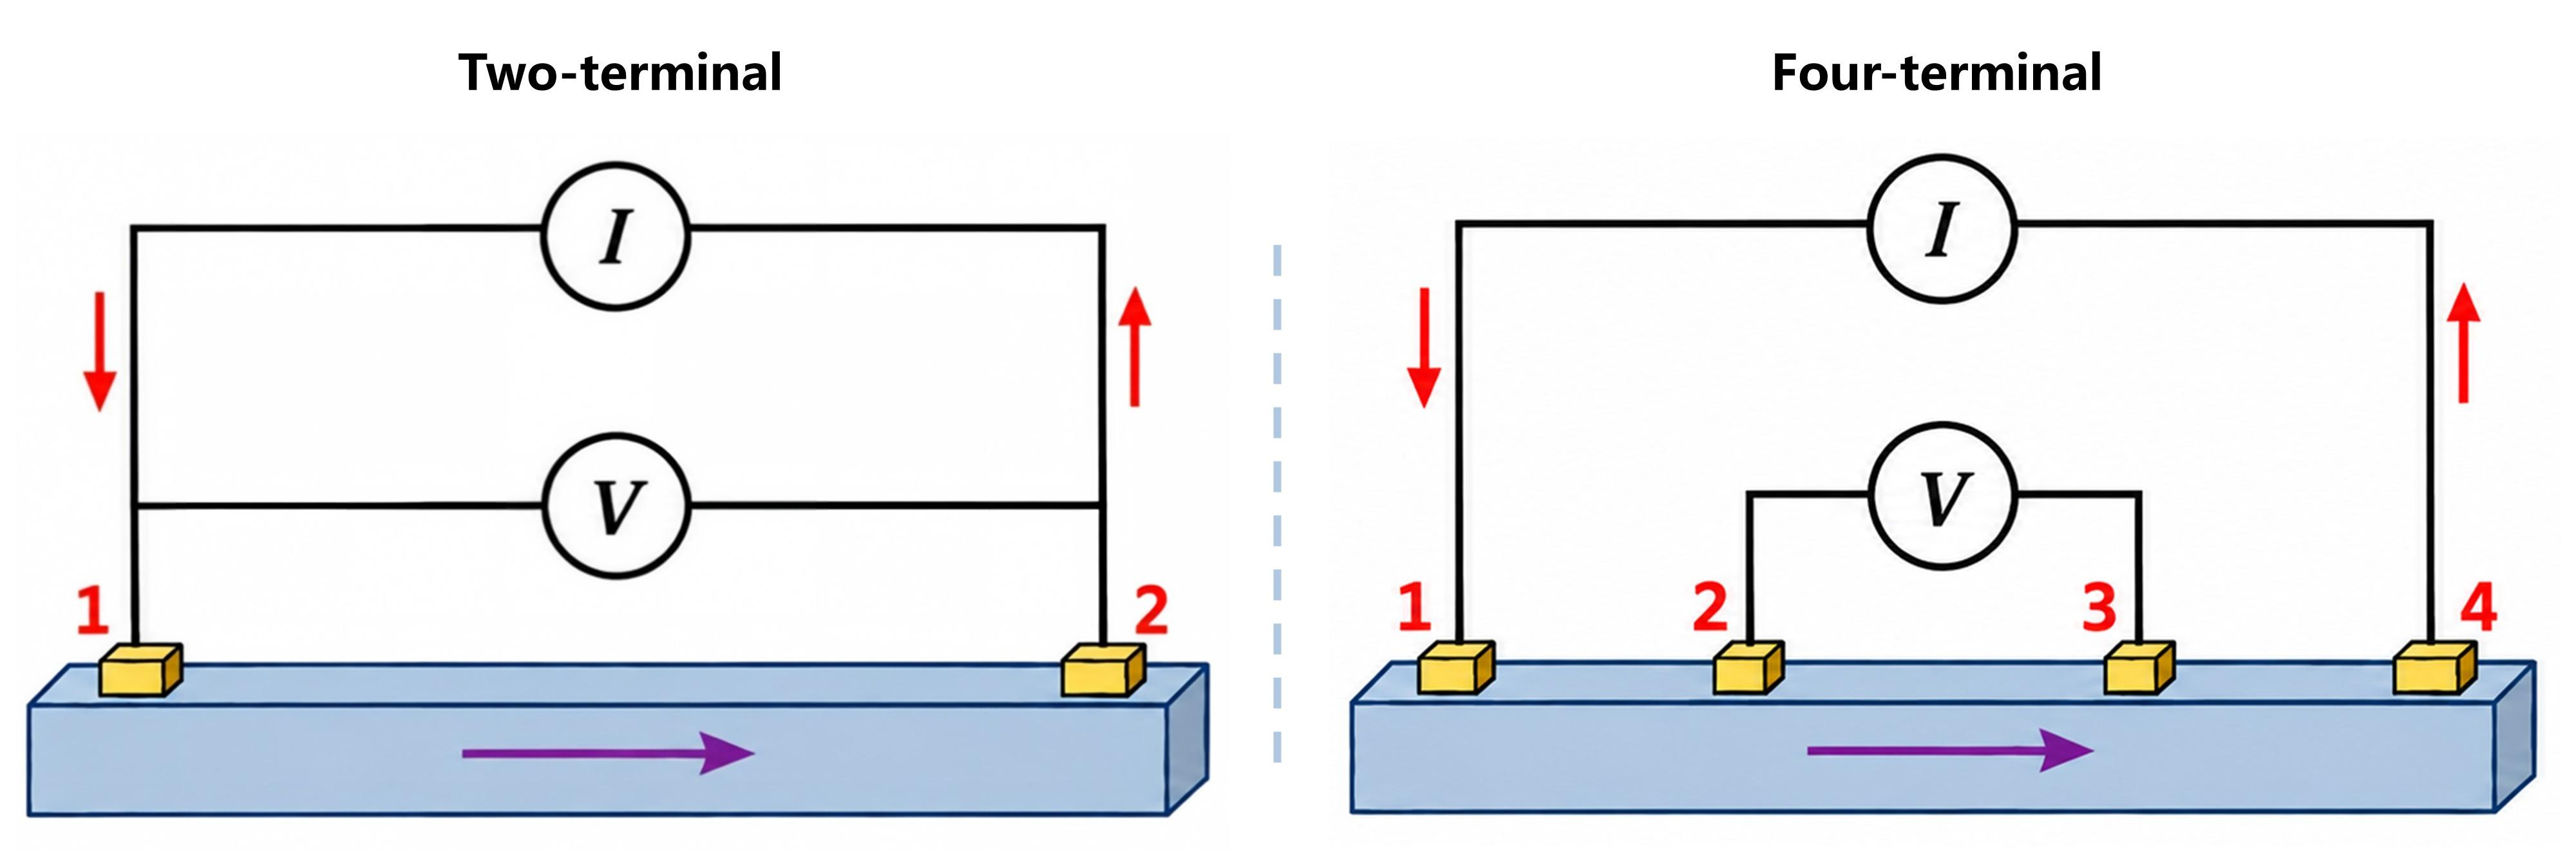
\includegraphics[width=0.95\textwidth]
    {12.jpg}

    \caption{两端法与四端法测量示意图}
    \label{fig:two-terminal}
\end{figure}

% ======================================================
% 2 四端法
% ======================================================

\section{四端法}

四端法（four-terminal method）采用四个独立电极，
其中两个电极用于通入电流，
另外两个电极用于测量电压。
其基本思想是将电流回路与电压测量回路分离，
从而显著降低接触电阻对测量结果的影响。

以四个电极依次标记为 1、2、3、4 为例，
可由外侧电极 1 和 4 通入电流 \(I_{14}\)，
并通过内侧电极 2 和 3 测量电压 \(V_{23}\)。
相应的四端电阻为

\[
R_{\mathrm{4P}}=\frac{V_{23}}{I_{14}}.
\]

由于电压测量支路与主电流回路分离，
而电压表通常具有很高的输入阻抗，
因此流过电压探针的电流近似为零。
在这种情况下，
电压电极的接触电阻不会产生显著的额外电压降。

四端法的主要作用可以概括为：
通过分离电流端和电压端，
减小或消除接触电阻造成的测量误差。

% ======================================================
% 3 霍尔棒法
% ======================================================

\section{霍尔棒法}

霍尔棒法（Hall bar method）采用具有规则几何结构的多电极样品，可以获得样品的方块电阻、电阻率、霍尔系数、载流子类型、载流子浓度 \(n\) 和载流子迁移率 \(\mu\)
等基本电学参数。

% ==================== Hall bar 示意图 ====================
\begin{figure}[htbp]
    \centering

    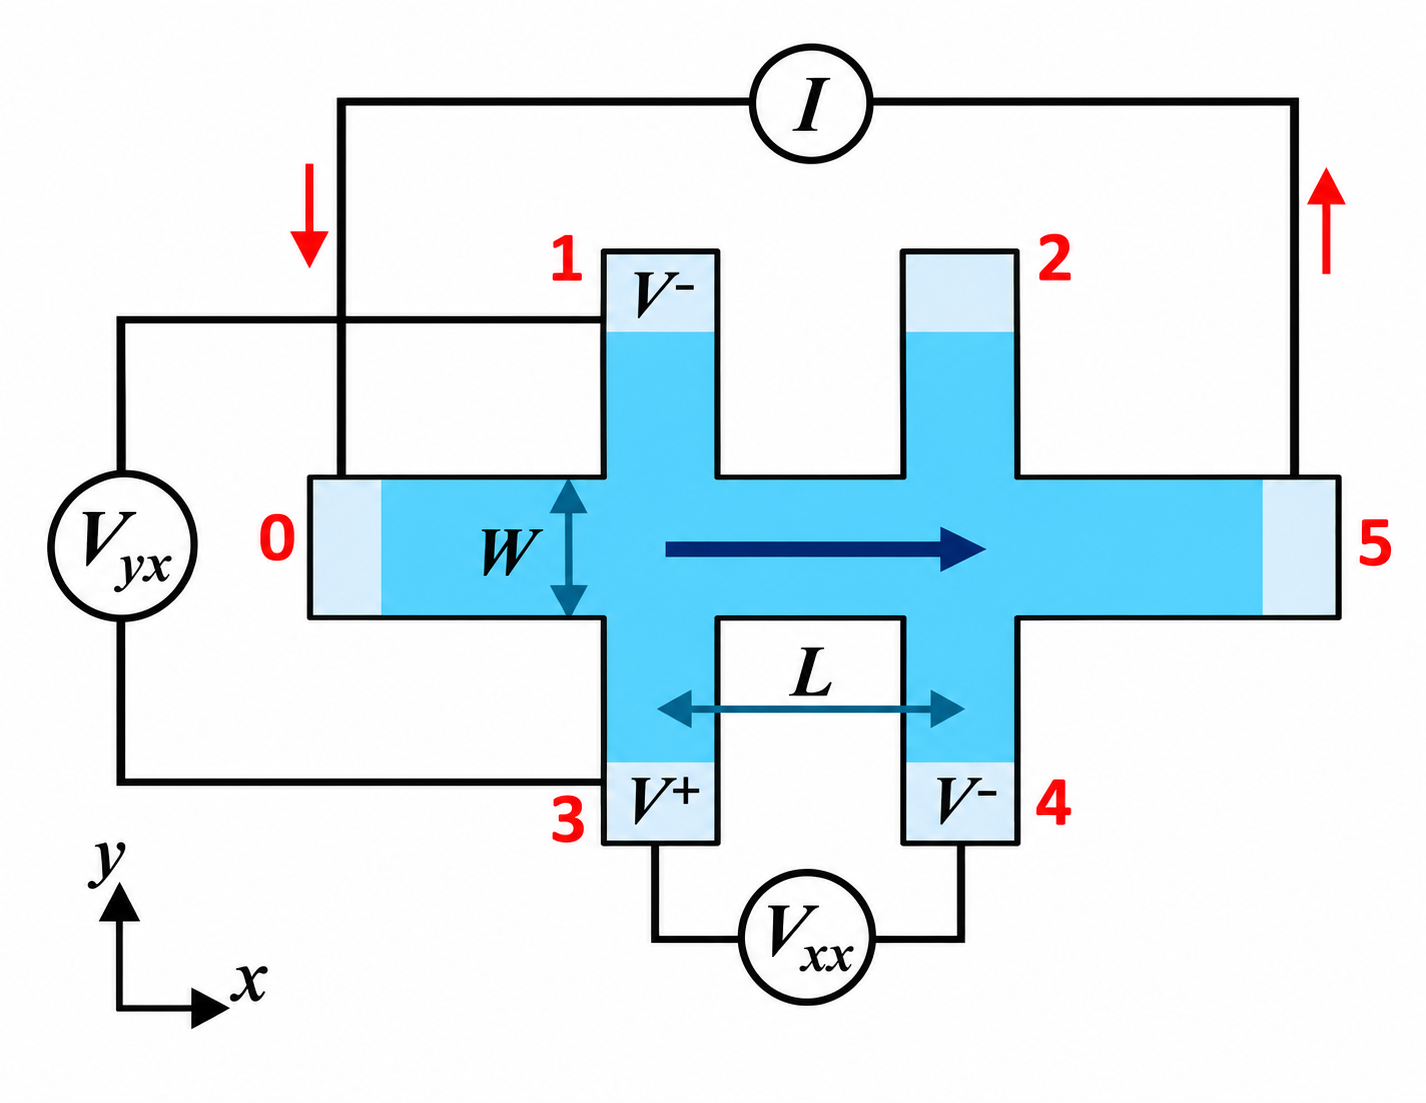
\includegraphics[width=0.6\textwidth]
    {3.png}
    
    \caption{Hall bar 法测量示意图}
    \label{fig:hall-bar}
\end{figure}

% ------------------------------------------------------

\subsection{纵向电输运}

对于 Hall bar 的纵向输运测量，
电流沿 \(x\) 方向流动，
纵向电压沿同一方向测量。

实验首先通过纵向电压与电流的比值得到纵向四端电阻：

\[
R_{xx}
=
\frac{V_{xx}}{I}.
\]

若两个纵向电压探针之间的距离为 \(L\)，
Hall bar 沟道宽度为 \(W\)，
则 \(L/W\) 表示两个电压探针之间所包含的方块数。
对于均匀二维薄膜，
纵向电阻与方块电阻 \(R_s\) 之间满足

\[
R_{xx}
=
R_s\frac{L}{W}.
\]

因此，Hall bar 的方块电阻可以由纵向四端电阻和沟道几何尺寸得到：

\[
R_s
=
R_{xx}\frac{W}{L}
=
\frac{V_{xx}}{I}\frac{W}{L}.
\]

其中，方块电阻 \(R_s\) 的单位通常表示为
\(\Omega/\square\)。

若进一步已知薄膜厚度 \(t\)，
则可以由方块电阻得到三维体电阻率：

\[
\rho_{xx}
=
R_s t
=
R_{xx}\frac{Wt}{L}.
\]

因此，Hall bar 纵向输运中的主要物理量之间满足

\[
R_{xx}=\frac{V_{xx}}{I},
\qquad
R_s=R_{xx}\frac{W}{L},
\qquad
\rho_{xx}=R_s t.
\]

% ------------------------------------------------------

\subsection{霍尔效应}

当电流沿 \(x\) 方向流过样品，
同时在垂直于样品表面的 \(z\) 方向施加磁场 \(B\) 时，
载流子受到洛伦兹力作用，
从而在横向 \(y\) 方向产生霍尔电压。

对于图中所示的测量几何，
电流沿 \(x\) 方向，
横向电压沿 \(y\) 方向测量，
因此实验测得的横向电压记为 \(V_{yx}\)。
相应的霍尔电阻为

\[
R_{yx}
=
\frac{V_{yx}}{I}.
\]

对于厚度为 \(t\) 的薄膜，
霍尔电阻率与测得的霍尔电阻之间满足

\[
\rho_{yx}
=
R_{yx}t.
\]

在普通霍尔效应占主导的情况下，
霍尔电阻率与磁场之间满足线性关系

\[
\rho_{yx}
=
R_H B,
\]

其中 \(R_H\) 为霍尔系数。
因此，霍尔电压可以写为

\[
V_{yx}
=
\frac{R_H I B}{t}.
\]

由此也可以得到

\[
R_{yx}
=
\frac{R_H}{t}B.
\]

因此，对于普通霍尔效应，
实验中通常测量 \(R_{yx}\) 随磁场 \(B\) 的变化，
并进行线性拟合：

\[
R_{yx}(B)
=
kB+b,
\qquad
k=\frac{dR_{yx}}{dB}.
\]

其中 \(k\) 为霍尔电阻对磁场的线性拟合斜率，
\(b\) 为由电极不完全对称、零场偏置等因素产生的截距。

由

\[
R_{yx}
=
\frac{R_H}{t}B
\]

可以得到霍尔系数

\[
R_H
=
t\frac{dR_{yx}}{dB}
=
tk.
\]

因此，对于厚度已知的薄膜，
霍尔系数可以直接由霍尔电阻--磁场曲线的斜率得到：

\[
R_H=tk.
\]

% ------------------------------------------------------

\subsection{载流子类型与载流子浓度}

在单一载流子近似下，
霍尔系数满足

\[
R_H
=
\frac{1}{nq},
\]

其中 \(n\) 为载流子浓度，
\(q\) 为载流子的电荷。

对于电子载流子，
\(q=-e\)，因此

\[
R_H
=
-\frac{1}{ne}.
\]

对于空穴载流子，
\(q=+e\)，因此

\[
R_H
=
\frac{1}{pe},
\]

其中 \(p\) 表示空穴浓度。

因此，在固定电压端定义和磁场正方向的条件下，
霍尔系数的符号可以用于判断主要载流子类型：

\[
R_H<0
\quad\Rightarrow\quad
\text{电子型载流子},
\qquad
R_H>0
\quad\Rightarrow\quad
\text{空穴型载流子}.
\]

由于薄膜厚度 \(t>0\)，
霍尔系数 \(R_H\) 与霍尔拟合斜率
\(k=dR_{yx}/dB\) 具有相同符号，
因此也可以直接根据 \(R_{yx}(B)\) 的斜率进行判断：

\[
k<0
\quad\Rightarrow\quad
\text{电子型载流子},
\qquad
k>0
\quad\Rightarrow\quad
\text{空穴型载流子}.
\]

需要注意的是，
霍尔信号的正负号同时取决于电压端定义、磁场正方向和电流方向。
因此，在利用霍尔信号判断载流子类型时，
必须首先统一实验中的电压、电流和磁场正方向。

对于单一载流子模型，
载流子浓度可以由霍尔系数得到：

\[
n
=
\frac{1}{e|R_H|}.
\]

结合 \(R_H=tk\)，
三维载流子浓度可以直接表示为

\[
n
=
\frac{1}{e\,t\,|k|}
=
\frac{1}
{e\,t\left|\dfrac{dR_{yx}}{dB}\right|}.
\]

若 \(t\) 采用 cm，
\(R_H\) 的单位为 \(\mathrm{cm^3/C}\)，
则得到的三维载流子浓度单位为
\(\mathrm{cm^{-3}}\)。

对于二维载流子系统，
还可以定义面载流子浓度 \(n_{\mathrm{2D}}\)。
由于

\[
R_{yx}
=
\frac{B}{n_{\mathrm{2D}}q},
\]

因此

\[
n_{\mathrm{2D}}
=
\frac{1}
{e\left|\dfrac{dR_{yx}}{dB}\right|}.
\]

三维载流子浓度与二维面载流子浓度之间满足

\[
n_{\mathrm{2D}}
=
nt.
\]

% ------------------------------------------------------

\subsection{载流子迁移率}

在单一载流子 Drude 模型下，
纵向电导率、载流子浓度和载流子迁移率之间满足

\[
\sigma_{xx}
=
ne\mu.
\]

因此，

\[
\mu
=
\frac{\sigma_{xx}}{ne}.
\]

在零磁场或霍尔角较小的情况下，
纵向电导率近似满足

\[
\sigma_{xx}
\simeq
\frac{1}{\rho_{xx}},
\]

因此迁移率可以写为

\[
\mu
=
\frac{1}{ne\rho_{xx}}.
\]

利用

\[
|R_H|
=
\frac{1}{ne},
\]

还可以得到常用的 Hall 迁移率表达式：

\[
\mu
=
\frac{|R_H|}{\rho_{xx}}.
\]

对于 Hall bar 薄膜，
利用
\(\rho_{xx}=R_s t\)
和
\(R_H=tk\)，
上述关系可以进一步写为

\[
\mu
=
\frac{|k|}{R_s}
=
\frac{1}{R_s}
\left|
\frac{dR_{yx}}{dB}
\right|.
\]

若进一步利用

\[
R_s
=
R_{xx}\frac{W}{L},
\]

则迁移率也可以直接由 Hall bar 的实验测量量表示为

\[
\mu
=
\left|
\frac{dR_{yx}}{dB}
\right|
\frac{L}{R_{xx}W}.
\]

因此，在单一载流子近似下，
Hall bar 测量得到的主要参数之间可以概括为

\[
R_H
=
t\frac{dR_{yx}}{dB},
\qquad
n
=
\frac{1}{e|R_H|},
\qquad
\mu
=
\frac{|R_H|}{\rho_{xx}}
=
\frac{\left|dR_{yx}/dB\right|}{R_s}.
\]

% ------------------------------------------------------

\subsection{电阻率张量与电导率张量}

当同时存在纵向和横向输运响应时，
电阻率和电导率需要采用张量形式描述。

按照实验几何定义，
\(x\) 方向为电流方向，
\(y\) 方向为横向响应方向，
因此实验上测得的是 \(\rho_{yx}\)。

对于二维各向同性 Hall 输运，
横向电阻率的两个非对角分量满足反对称关系

\[
\rho_{yx}
=
-\rho_{xy}.
\]

因此，\(\rho_{xy}\) 与 \(\rho_{yx}\) 的绝对值相同，
但符号相反。

以下在张量表达式中统一采用 \(xy\) 记号，
电阻率张量写为

\[
\rho
=
\sigma^{-1}
=
\begin{pmatrix}
\rho_{xx} & \rho_{xy} \\
-\rho_{xy} & \rho_{xx}
\end{pmatrix}.
\]

由电阻率张量与电导率张量之间的逆矩阵关系，
电导率张量为

\[
\sigma
=
\frac{1}
{\rho_{xx}^{2}+\rho_{xy}^{2}}
\begin{pmatrix}
\rho_{xx} & -\rho_{xy} \\
\rho_{xy} & \rho_{xx}
\end{pmatrix}.
\]

因此，纵向和横向电导率分别为

\[
\sigma_{xx}
=
\frac{\rho_{xx}}
{\rho_{xx}^{2}+\rho_{xy}^{2}},
\qquad
\sigma_{xy}
=
-\frac{\rho_{xy}}
{\rho_{xx}^{2}+\rho_{xy}^{2}}.
\]

若实验数据采用 \(\rho_{yx}\) 记号，
则应利用

\[
\rho_{yx}
=
-\rho_{xy}
\]

进行相应的符号转换。

% ------------------------------------------------------

\subsection{磁阻的对称化与霍尔信号的反对称化}

实际输运测量中，
由于电极位置难以做到完全理想，
纵向与横向信号之间可能发生一定程度的混合。
例如，横向电压探针若存在轻微纵向错位，
测得的 Hall 信号中会混入部分纵向电阻成分。

因此，在完成正、负磁场扫描后，
可以利用纵向和横向输运分量关于磁场方向的不同对称性，
提取相应的真实输运信号。

对于纵向电阻，
采用对称化处理：

\[
R_{xx}(B)
=
\frac{
R'_{xx}(B)+R'_{xx}(-B)
}{2}.
\]

纵向磁阻主要对应磁场的偶对称分量。

对于霍尔电阻，
采用反对称化处理：

\[
R_{yx}(B)
=
\frac{
R'_{yx}(B)-R'_{yx}(-B)
}{2}.
\]

霍尔信号主要对应磁场的奇对称分量。

因此，实际计算霍尔系数时，
通常首先对原始横向电阻进行反对称化，
再对得到的 \(R_{yx}(B)\) 进行线性拟合：

\[
R_{yx}(B)
=
kB+b,
\qquad
k=\frac{dR_{yx}}{dB}.
\]

随后依次得到

\[
R_H=tk,
\qquad
n=\frac{1}{e|R_H|},
\qquad
\mu=\frac{|k|}{R_s}.
\]

% ======================================================
% 4 范德堡法
% ======================================================

\section{范德堡法}

范德堡法（van der Pauw method）
是一种基于四个边缘电极的薄膜电输运测量方法。
该方法既可以测量方块电阻，
也可以进行霍尔效应测量。

适用于 van der Pauw 测量的样品需要满足一定条件：
样品厚度均匀、面内近似各向同性、内部无孔洞；
四个欧姆接触电极应位于样品边缘，
且电极接触面积应远小于样品总面积。

% ==================== van der Pauw 示意图 ====================
\begin{figure}[htbp]
    \centering

    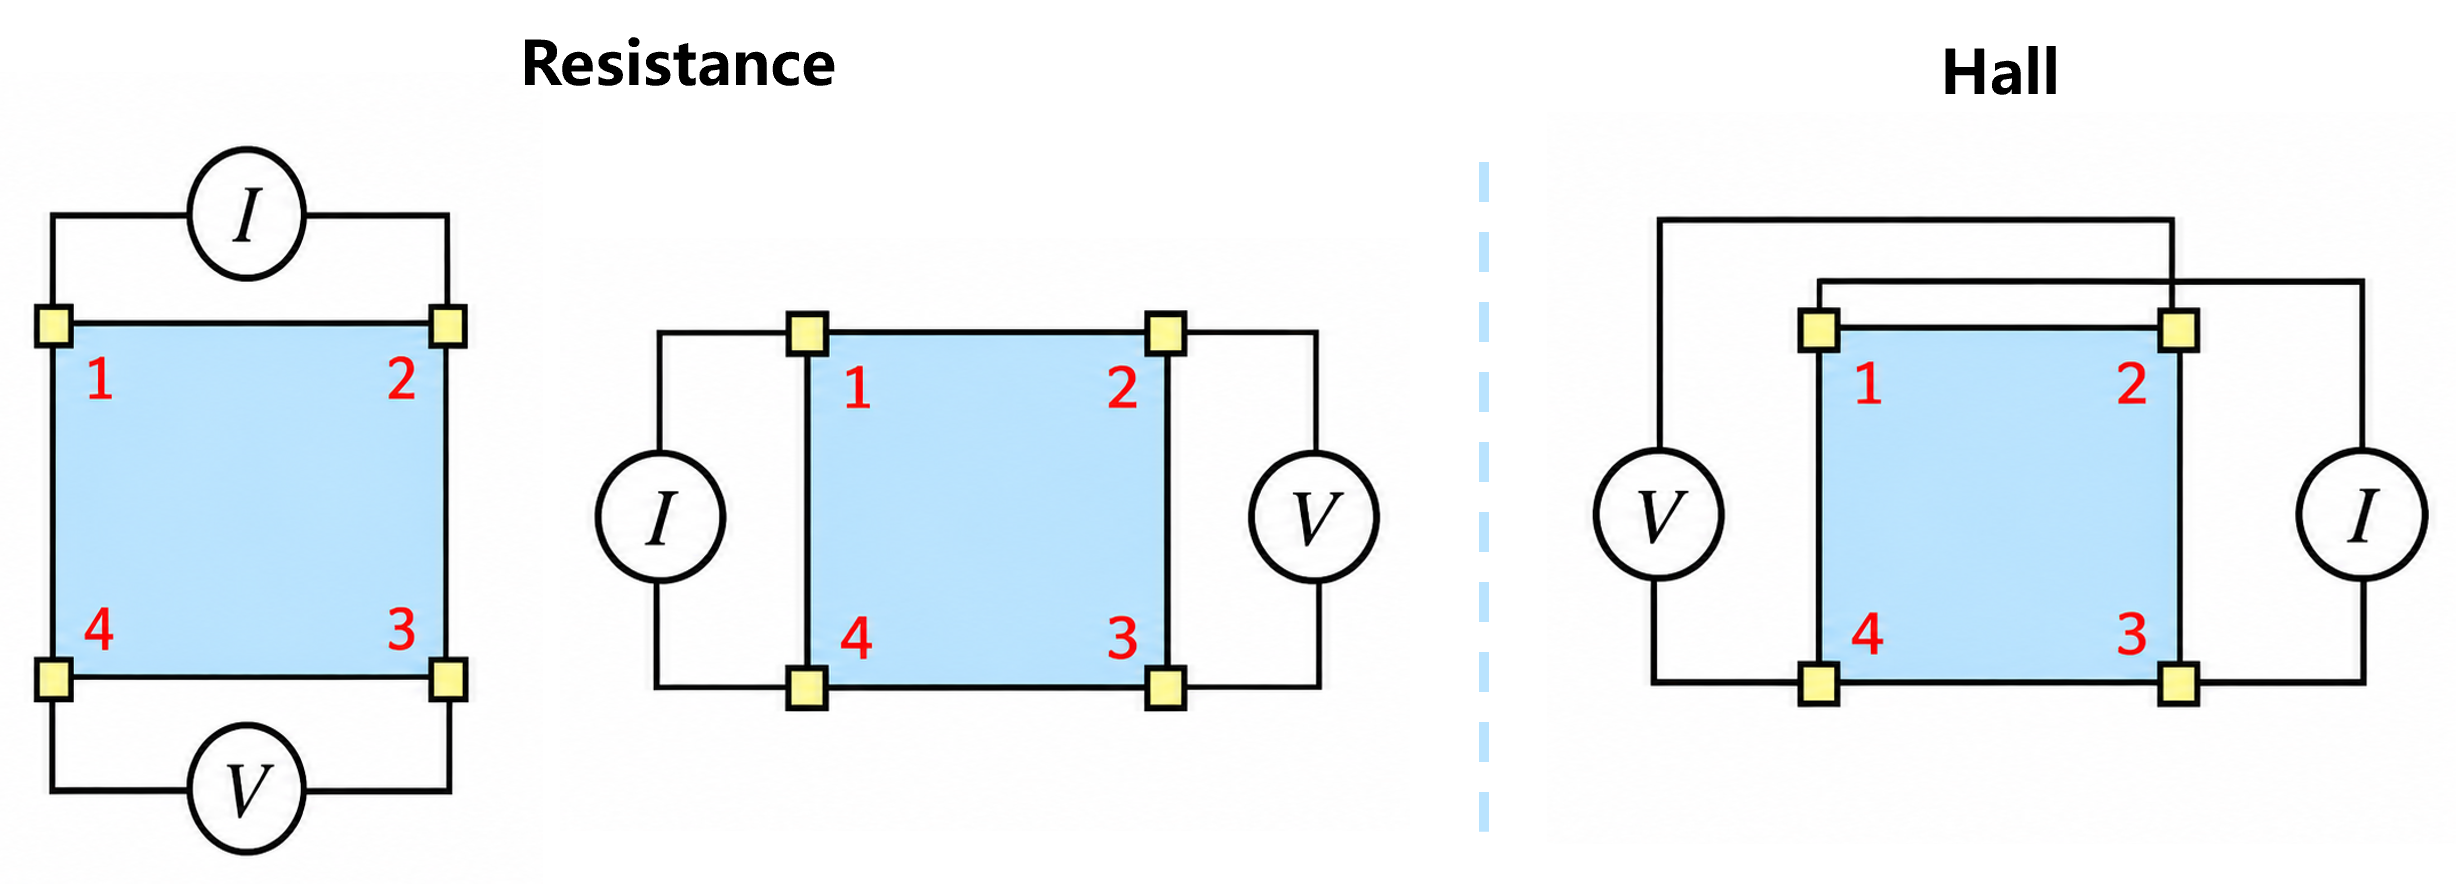
\includegraphics[width=0.9\textwidth]{4.png}

    \caption{范德堡法测量示意图}
    \label{fig:van-der-pauw}
\end{figure}

% ------------------------------------------------------

\subsection{方块电阻测量}

设样品边缘的四个电极依次编号为
1、2、3、4。

首先在相邻电极 1 和 2 之间通入电流 \(I_{12}\)，
并测量另外两个相邻电极 3 和 4 之间的电压 \(V_{34}\)，
定义第一组电阻为

\[
R_A
=
\frac{V_{34}}{I_{12}}.
\]

随后在相邻电极 1 和 4 之间通入电流 \(I_{14}\)，
并测量另外两个相邻电极 2 和 3 之间的电压 \(V_{23}\)，
定义第二组电阻为

\[
R_B
=
\frac{V_{23}}{I_{14}}.
\]

这两组电阻分别反映样品在两个等效测量方向上的
电输运响应。

定义两组电阻之比为

\[
Q
=
\frac{R_A}{R_B}.
\]

由 \(Q\) 可以进一步计算范德堡修正因子 \(f\)。

% ------------------------------------------------------

\subsection{范德堡修正因子}

范德堡修正因子 \(f\)
用于修正 \(R_A\) 与 \(R_B\) 不完全相等所带来的影响。

电阻比 \(Q\) 与修正因子 \(f\) 之间满足

\[
\frac{Q-1}{Q+1}
=
\frac{f}{\ln 2}
\operatorname{arccosh}
\left[
\frac{1}{2}
\exp\left(
\frac{\ln 2}{f}
\right)
\right],
\qquad
Q=\frac{R_A}{R_B}.
\]

由实验测得 \(R_A\) 和 \(R_B\) 后，
首先计算 \(Q\)，
随后根据上述关系求解修正因子 \(f\)。

获得 \(f\) 后，
方块电阻 \(R_s\) 写为

\[
R_s
=
\frac{\pi}{\ln 2}
\frac{R_A+R_B}{2}
f.
\]

因此，
范德堡方块电阻的数据处理过程可以概括为

\[
R_A,\;R_B
\;\longrightarrow\;
Q=\frac{R_A}{R_B}
\;\longrightarrow\;
f
\;\longrightarrow\;
R_s.
\]

当 \(R_A\) 与 \(R_B\) 越接近时，
样品在两个测量方向上的输运响应越接近，
修正因子 \(f\) 也相应趋近于 1。

实验中若 \(R_A\) 与 \(R_B\) 存在明显差异，
则应根据上述关系计算实际修正因子，
而不能直接忽略该修正。

% ------------------------------------------------------

\subsection{范德堡法的霍尔测量}

范德堡结构还可以用于霍尔效应测量。

首先在垂直于薄片表面的方向施加磁场 \(B\)，
随后在对角电极 1 和 3 之间通入电流 \(I_{13}\)，
并测量另外两个对角电极 2 和 4 之间的电压 \(V_{24}\)。

为了消除热电势、不等位电势等副效应，
需要同时改变磁场方向和电流方向，
分别测量以下四组电压：

\[
V_{24}(+B,+I),\qquad
V_{24}(+B,-I),\qquad
V_{24}(-B,+I),\qquad
V_{24}(-B,-I).
\]

由四组数据组合得到霍尔电压：

\[
V_H
=
\frac{
\left|
V_{24}(+B,+I)
-
V_{24}(+B,-I)
-
V_{24}(-B,+I)
+
V_{24}(-B,-I)
\right|
}{4}.
\]

相应的霍尔电阻为

\[
R_{yx}
=
\frac{V_H}{I_{13}}.
\]

这种同时改变磁场方向和电流方向的测量方式，
主要用于消除热电势、不等位电势等副效应，
从而提取真正的霍尔响应。

\end{document}

\end{document}